\documentclass{article}
\usepackage{siunitx}
%% Language and font encodings
\usepackage[english]{babel}
\usepackage[utf8x]{inputenc}
\usepackage[T1]{fontenc}
\usepackage{longtable}
\usepackage{multirow}

%% Sets page size and margins
\usepackage[a4paper,top=3cm,bottom=2cm,left=3cm,right=3cm,marginparwidth=1.75cm]{geometry}

%% Useful packages
\usepackage{amsmath}
\usepackage{graphicx,float}
\usepackage[colorinlistoftodos]{todonotes}
\usepackage[colorlinks=true, allcolors=blue]{hyperref}

\title{CSP334: Computer Networks \linebreak
Lab Assignment No 4\linebreak
Http Wireshark Assignment}
\author{Abhishek Gupta  2016UCS0012}

\begin{document}
\maketitle

\section{SET 1}

\subsection{Q1}
My browser is running HTTP version 1.1. Server is also running HTTP version 1.1\\
\subsection{Q2}
My browser indicates that it can accept en-GB (English, Great Britain) to the server\\
\subsection{Q3}
IP Address of my computer is 10.10.41.239. IP Address of cncourse web server is 145.14.144.77. You can see it in request message from my computer to cncourse web server\\
\subsection{Q4}
Status code returned from the server was 200.\\
Status Message was OK.\\
  \begin{figure}[H]
 \centering
 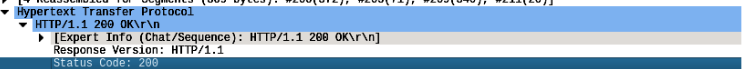
\includegraphics[width=0.8\textwidth]{../Set1/q4/a.png}
 \caption{\label{fig:PING}Screenshot of http Get file}
 \end{figure}
\subsection{Q5}
We can filter messages by http.last-modified and we see that the HTTP response I received for the html file doesn’t show this field. However as seen in screenshot my ocsp responce has a last modified field with value of :\\
Last-Modified: Sun, 16 Sep 2018 01:08:55 GMT\\
  \begin{figure}[H]
 \centering
 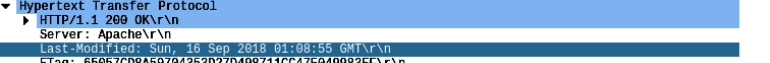
\includegraphics[width=0.8\textwidth]{../Set1/q5/a.png}
 \caption{\label{fig:PING}Screenshot of http Get file}
 \end{figure}
\subsection{Q6}
HTML file sent by cncourse server is of 680 bytes\\
\subsection{Q7}
No.The raw data appears to match up exactly with what is shown in thepacket-listing window.\\
\subsection{Q8}
A total of 4 requests were sent by my browser as shown in screenshot. Server responded with 2 responses.\\
  \begin{figure}[H]
 \centering
 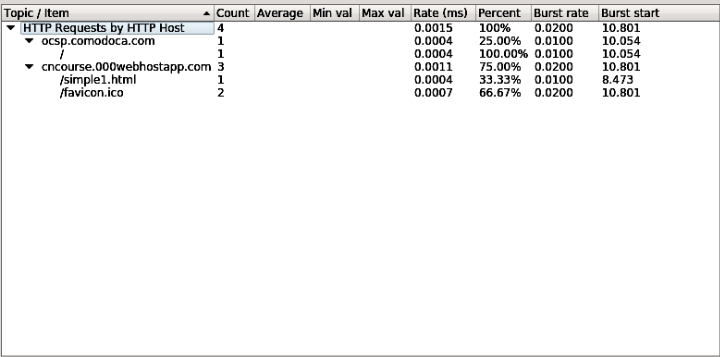
\includegraphics[width=0.8\textwidth]{../Set1/q8/a.png}
 \caption{\label{fig:PING}Screenshot of http Get file}
 \end{figure}
\subsection{Q9}
  \begin{figure}[H]
 \centering
 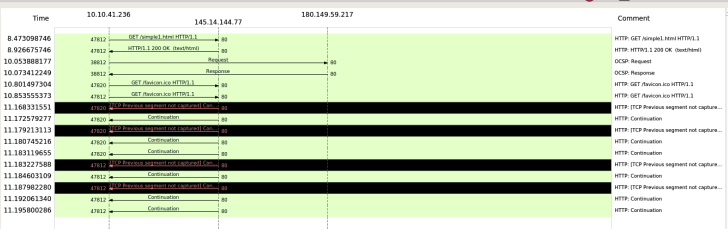
\includegraphics[width=0.8\textwidth]{../Set1/q9/a.png}
 \caption{\label{fig:PING}Screenshot of http Get file}
 \end{figure}
\subsection{Q10}
Last-Modified: Fri, 03 Jun 2016 13:32:18 GMT. This last modified field is for gif image.\\
No. of bytes for html file = 868 bytes\\
No. of bytes for image = 9601 bytes\\
Therefore total bytes returned to browser = 10469 bytes.\\
Total of 7 http requests were sent and 7 responses were registered from server.\\
  \begin{figure}[H]
 \centering
 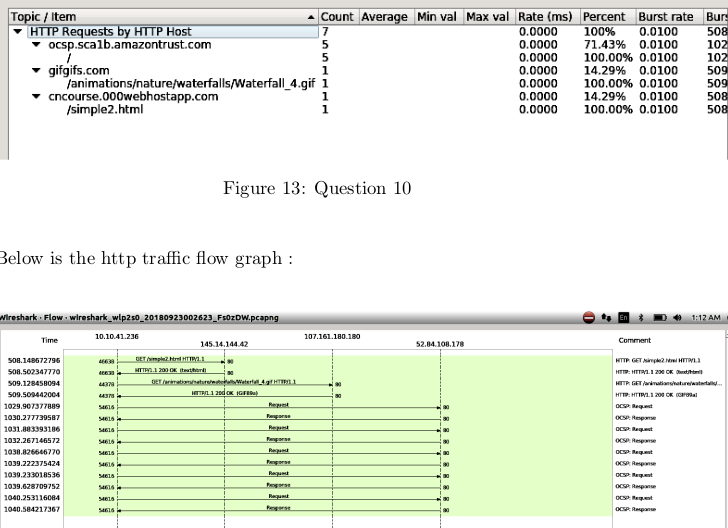
\includegraphics[width=0.8\textwidth]{../Set1/q10/a.png}
 \caption{\label{fig:PING}Screenshot of http Get file}
 \end{figure}
\subsection{Q11}
  \begin{figure}[H]
 \centering
 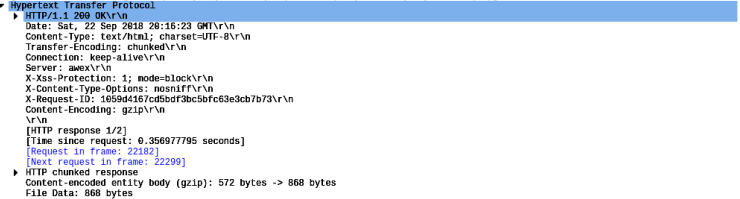
\includegraphics[width=0.8\textwidth]{../Set1/q11/a.png}
 \caption{\label{fig:PING}Screenshot of http Get file}
 \end{figure}
\subsection{Q12}
  \begin{figure}[H]
 \centering
 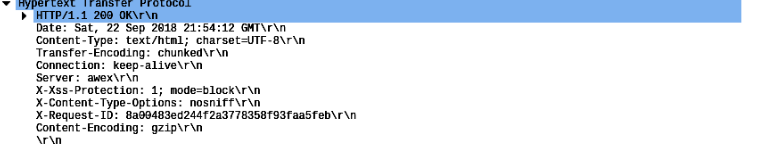
\includegraphics[width=0.8\textwidth]{../Set1/q12/a.png}
 \caption{\label{fig:PING}Screenshot of http Get file}
 \end{figure}
 
   \begin{figure}[H]
 \centering
 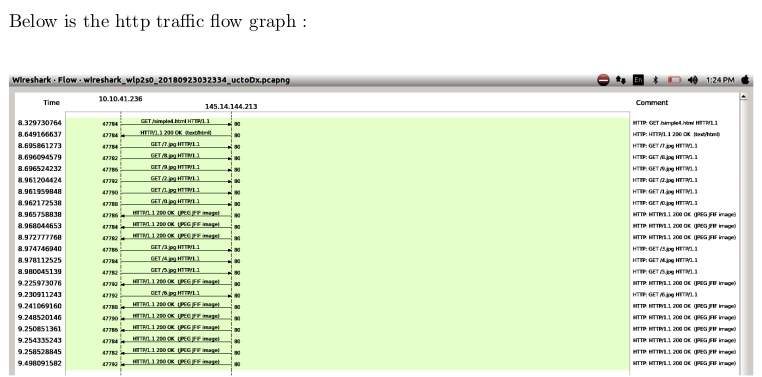
\includegraphics[width=0.8\textwidth]{../Set1/q12/b.png}
 \caption{\label{fig:PING}Screenshot of http Get file}
 \end{figure}
\subsection{Q13}
The time required to access the file is 2.754 - 1.952 = 0.802 seconds or 802 ms.\\
\subsection{Q14}
File              Value\\
Source Port No.23\\
DestinationPort 47360\\
No.Header Length 32 bytes\\
Acknowledgement 119\\
No.Reserved  0(Not set)\\
Flags 24\\
Window Size  227\\
TCP Checksum 62287\\
Urgent Pointer 0\\
Options 12 bytes\\
Data1 byte, 61\\
\section{SET 2}

\subsection{Q1}
No I don’t see any IF-MODIFIED-SINCE line in http GET request as you can see in the following screenshot.\\
  \begin{figure}[H]
 \centering
 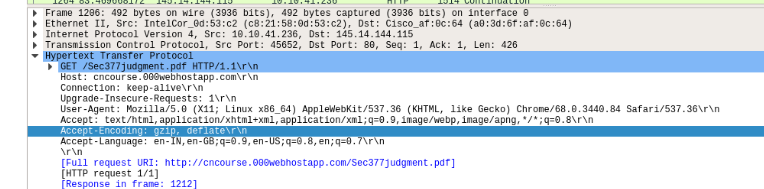
\includegraphics[width=0.8\textwidth]{../Set2/q1/a.png}
 \caption{\label{fig:PING}Screenshot of http Get file}
 \end{figure}
\subsection{Q2}
The server did not explicitly send teh contents of the file as I was requesting a pdf file in my request. However it sents that media type teht it is going to send is of type pdf as you can see in screenshot.\\
\subsection{Q3}
Yes,I see an IF-MODIFIED-SINCE: line in the HTTP GET request header.\\
\subsection{Q4}
HTTP status code and message sent by server in response to this is 304 Not Modified. Server did not explicitly return anything in response of teh GET message.\\
It’s because there is a proxy server which has this information already stored.In GET request browser asks if the file requested has been modified since a particular date, if not modified do not return anything to the server as this information is already with us.\\
  \begin{figure}[H]
 \centering
 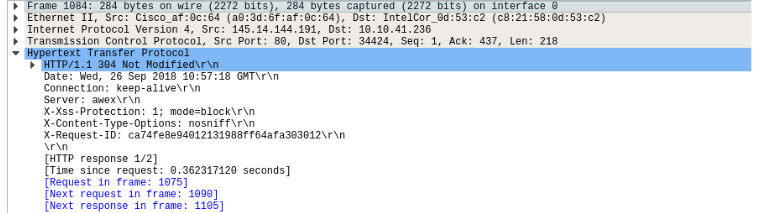
\includegraphics[width=0.8\textwidth]{../Set2/q4/a.png}
 \caption{\label{fig:PING}Screenshot of http Get file}
 \end{figure}
\section{SET 3}

\subsection{Q1}
Long File: \\
1 http GET request was sent by my browser to cncourse server. Packet Number 66 is the GET request message. \\
  \begin{figure}[H]
 \centering
 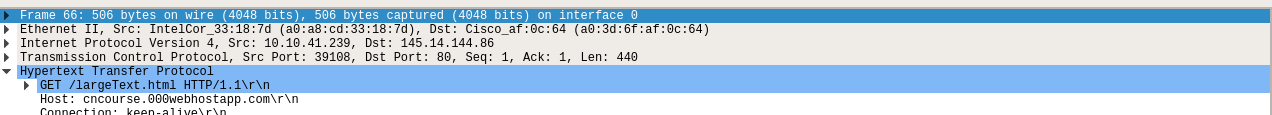
\includegraphics[width=0.8\textwidth]{../Set3/q1/a.png}
 \caption{\label{fig:PING}Screenshot of http Get file}
 \end{figure}
 
 PDF File:\\
2 http GET request messages were sent by my browser. Packet numbers 83 and 3124 are the two GET requests.\\

  \begin{figure}[H]
 \centering
 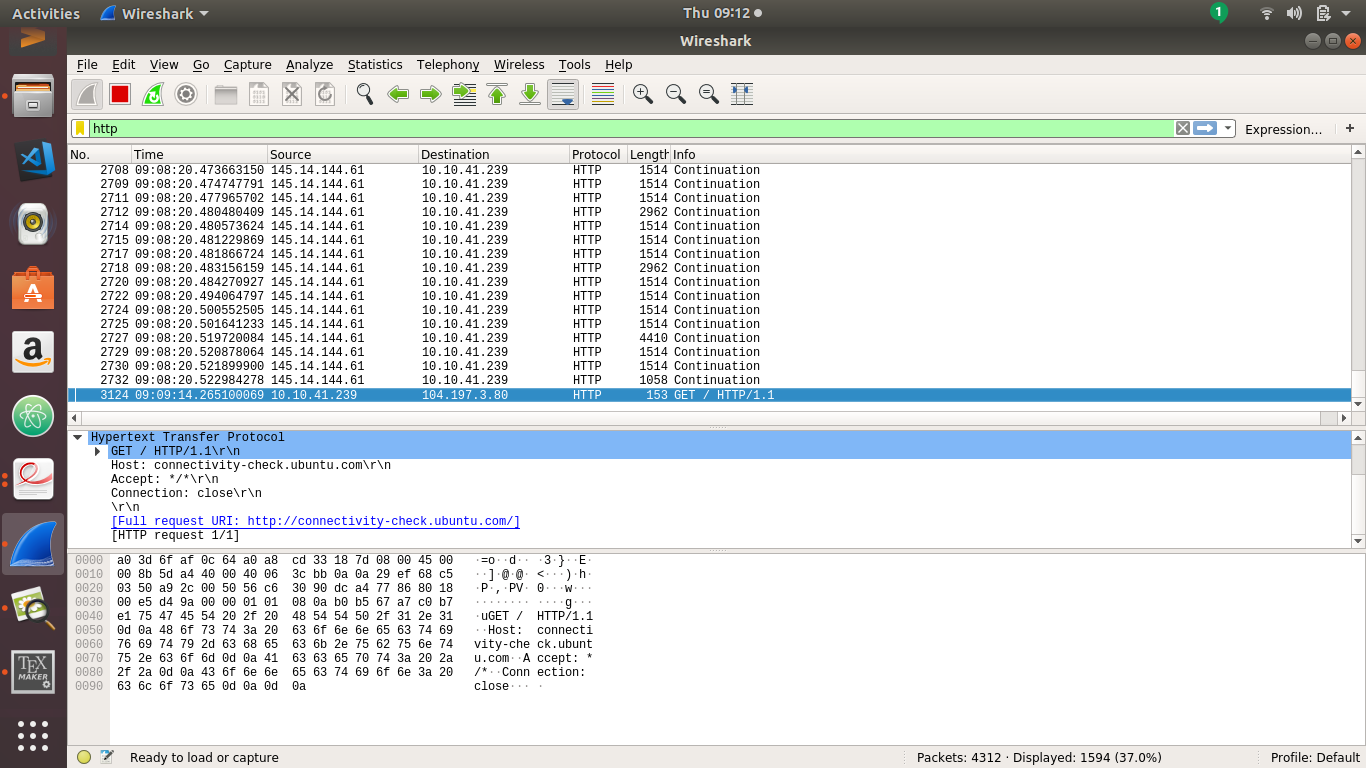
\includegraphics[width=0.8\textwidth]{../Set3/q1/b.png}
 \caption{\label{fig:PING}Screenshot of http Get file}
 \end{figure}
 
   \begin{figure}[H]
 \centering
 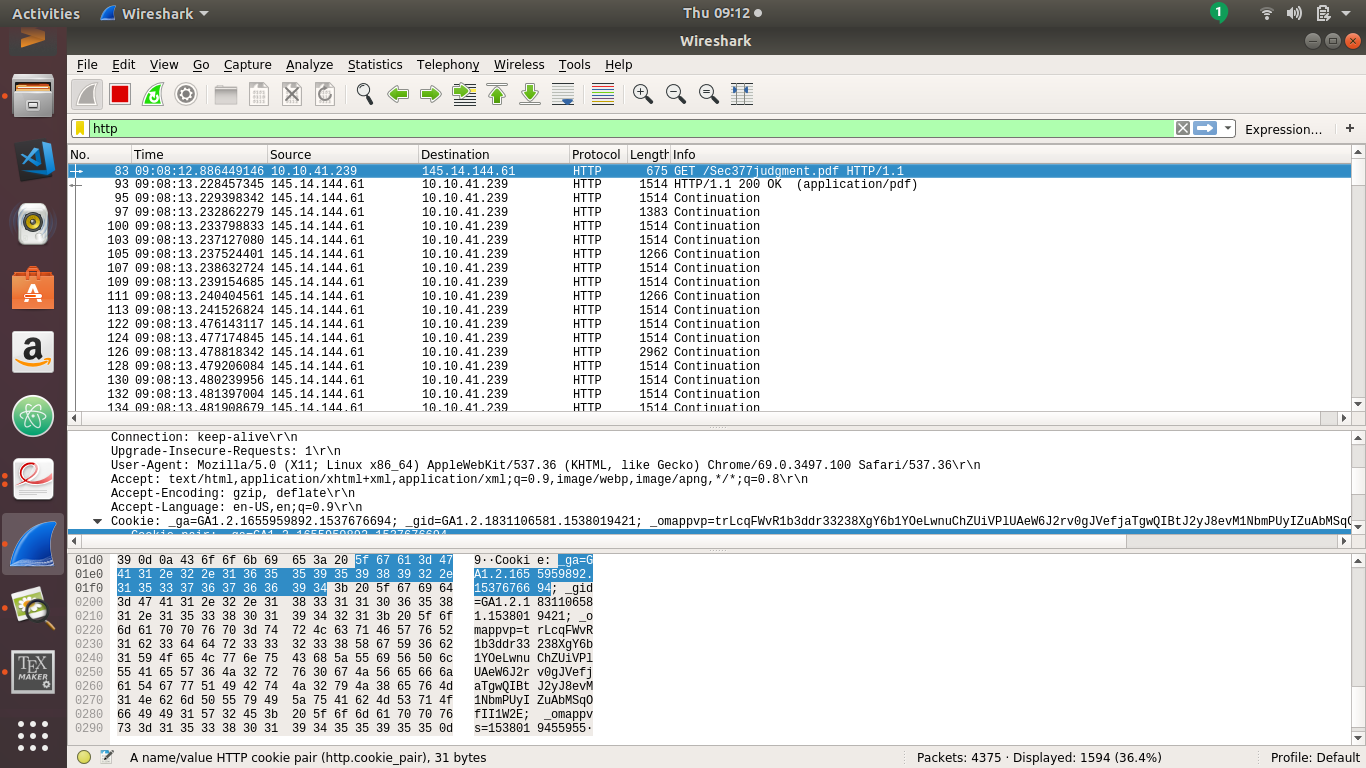
\includegraphics[width=0.8\textwidth]{../Set3/q1/c.png}
 \caption{\label{fig:PING}Screenshot of http Get file}
 \end{figure}

\subsection{Q2}

Long File: \\
Packet number 73 contains the stauts code 200 and phrase associated with it that is OK.\\
  \begin{figure}[H]
 \centering
 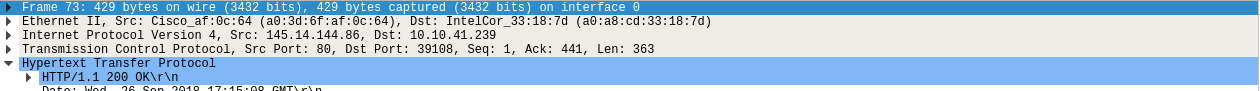
\includegraphics[width=0.8\textwidth]{../Set3/q2/a.png}
 \caption{\label{fig:PING}Screenshot of http Get file}
 \end{figure}
 
 Long File: \\
Packet number 93 contains the stauts code 200 and phrase associated with it that is OK.\\
  \begin{figure}[H]
 \centering
 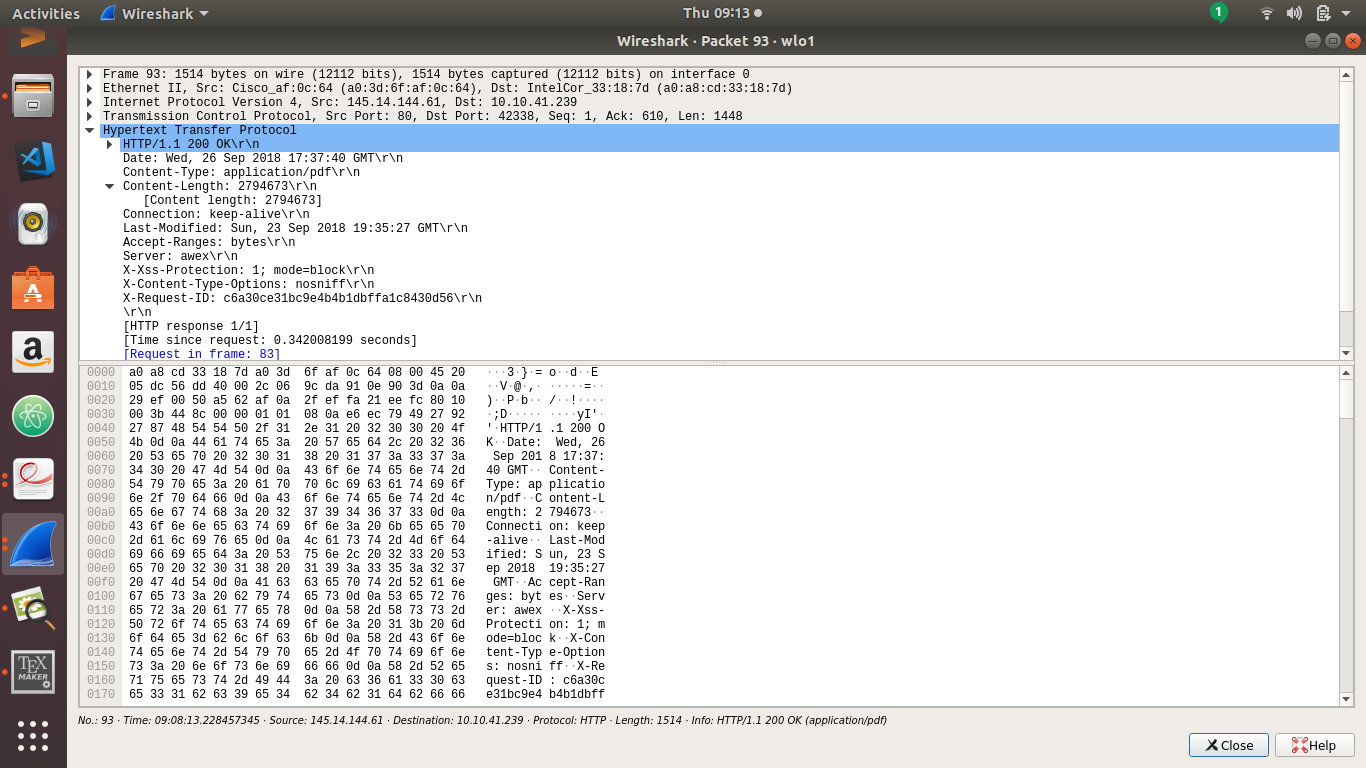
\includegraphics[width=0.8\textwidth]{../Set3/q2/b.png}
 \caption{\label{fig:PING}Screenshot of http Get file}
 \end{figure}
\subsection{Q3}
Long File:\\
Status Code : 200\\
Phrase : OK\\

Pdf File:\\
Status Code : 200\\
Phrase : OK\\

\subsection{Q4}
In my case, HTTP Continuation responses carried the long text file on the
server. I tried to change the same as demostrated on internet by going on
”edit” option in wireshark and select ”preferences option”, then selecting ”tcp”
and checking some boxes but that didn’t worked out for me. A total of 246
continuation responses were registered in case of content from wikipedia page.\\

  \begin{figure}[H]
 \centering
 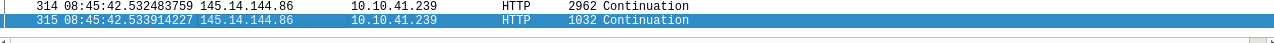
\includegraphics[width=0.8\textwidth]{../Set3/q4/a1.png}
 \caption{\label{fig:PING}Screenshot of http Get file}
 \end{figure}
 
   \begin{figure}[H]
 \centering
 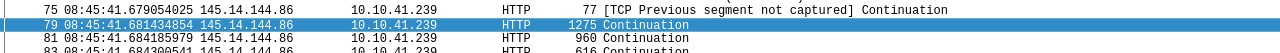
\includegraphics[width=0.8\textwidth]{../Set3/q4/a2.png}
 \caption{\label{fig:PING}Screenshot of http Get file}
 \end{figure}
 
 As in above case, there are also many continuations http response messages.\\
\section{SET 4}

\subsection{Q1}
Three HTTP messages were sent by my browser. First one is HTTP GET request
to open the the html page.Second one is also HTTP GET request to get favicon. Third one was HTTP POST message to post the form that we just filled.You can see these requests in the given screenshot.\\

 \begin{figure}[H]
 \centering
 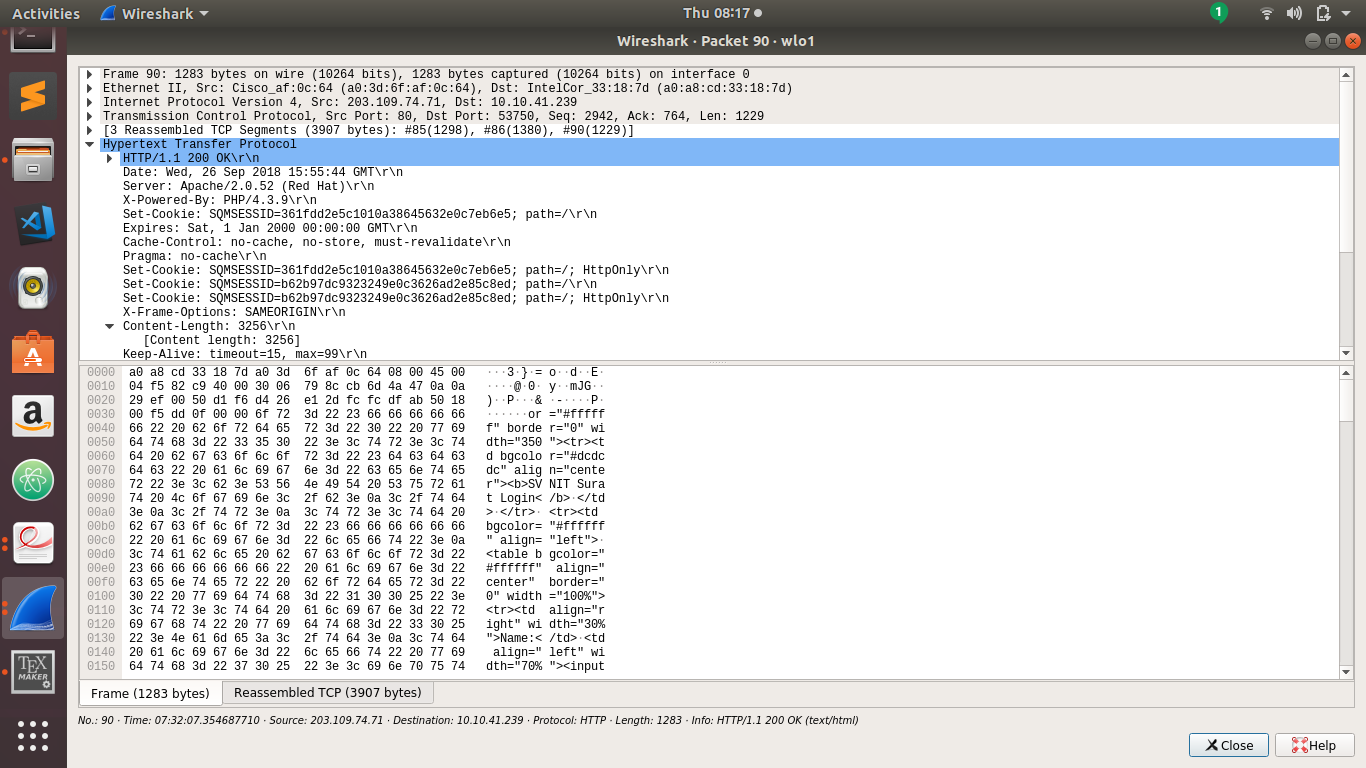
\includegraphics[width=0.8\textwidth]{../Set5/q1/a.png}
 \caption{\label{fig:PING}Screenshot of tcpdump file}
 \end{figure}
 
  \begin{figure}[H]
 \centering
 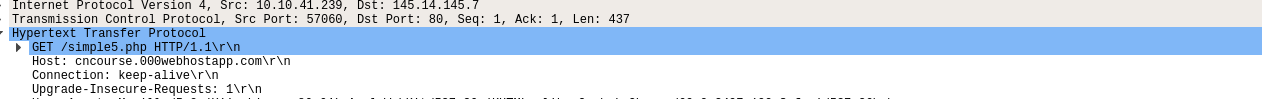
\includegraphics[width=0.8\textwidth]{../Set4/a.png}
 \caption{\label{fig:PING}Screenshot of http Get file}
 \end{figure}
 
  \begin{figure}[H]
 \centering
 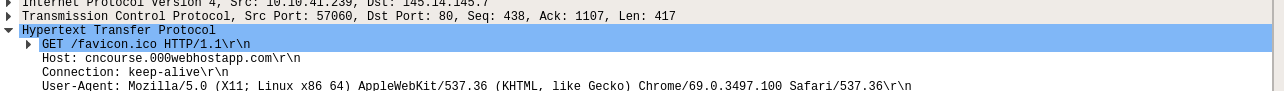
\includegraphics[width=0.8\textwidth]{../Set4/b.png}
 \caption{\label{fig:PING}Screenshot of http Get favicon}
 \end{figure}
 
  \begin{figure}[H]
 \centering
 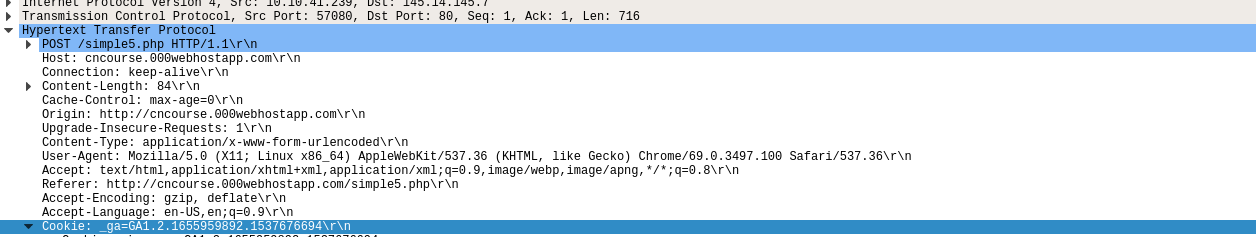
\includegraphics[width=0.8\textwidth]{../Set4/c.png}
 \caption{\label{fig:PING}Screenshot of http Post}
 \end{figure}
 
   \begin{figure}[H]
 \centering
 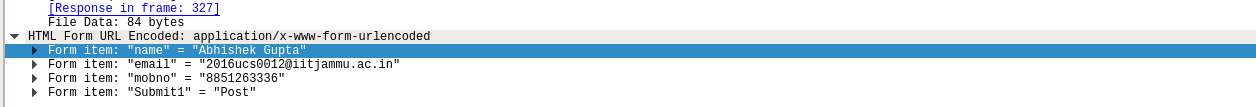
\includegraphics[width=0.8\textwidth]{../Set4/d.png}
 \caption{\label{fig:PING}Screenshot of Form}
 \end{figure}

The requests were sent to cncourse web server (145.14.145.7)\\
\section{SET 5}

\subsection{Q1}
In response to the initial HTTP GET message from my browser, server’s re-
sponse was 200 OK. You can see this in the screenshot above.\\

 \begin{figure}[H]
 \centering
 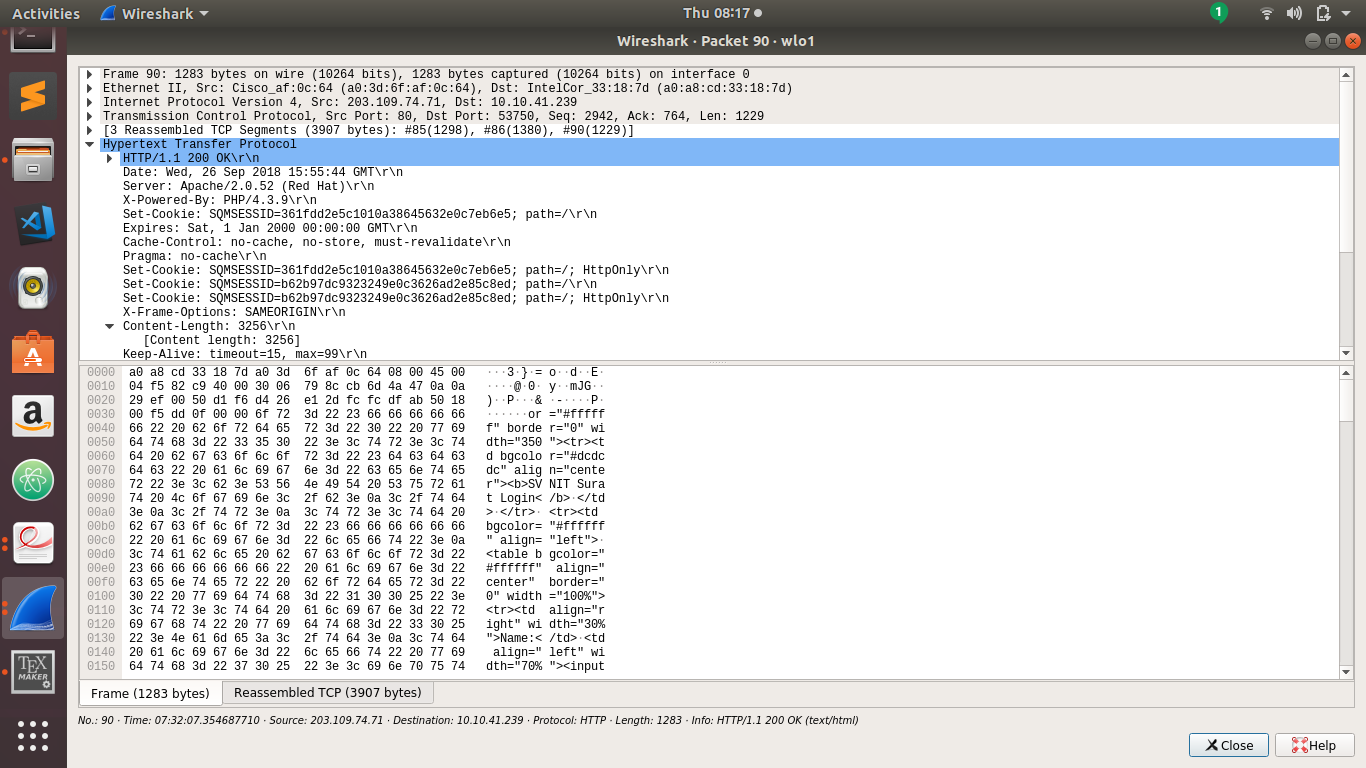
\includegraphics[width=0.8\textwidth]{../Set5/q1/a.png}
 \caption{\label{fig:PING}Screenshot of tcpdump file}
 \end{figure}
 
\subsection{Q2}

 \begin{figure}[H]
 \centering
 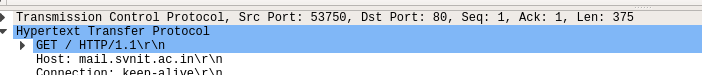
\includegraphics[width=0.8\textwidth]{../Set5/q2/a.png}
 \caption{\label{fig:PING}previous http get request}
 \end{figure}
 
  \begin{figure}[H]
 \centering
 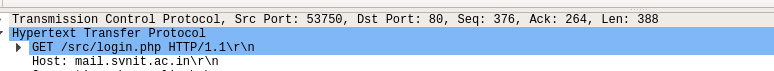
\includegraphics[width=0.8\textwidth]{../Set5/q2/b.png}
 \caption{\label{fig:PING}New http get request}
 \end{figure}

When my browser sends the HTTP GET message for the second time, the new
field added is Cookie. Cookie: SQMSESSID=b62b97dc9323249e0c3626ad2e85c8ed
You can see this highlighted in the below given screenshot: \\
 

 \begin{figure}[H]
 \centering
 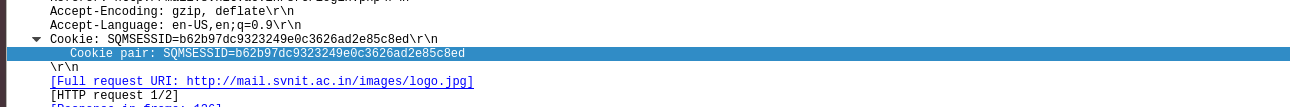
\includegraphics[width=0.8\textwidth]{../Set5/q2/c.png}
 \caption{\label{fig:PING}Screenshot of cookie}
 \end{figure}

\subsection{Q3}
You can see the highlighted password which I found in POST request \\
 \begin{figure}[H]
 \centering
 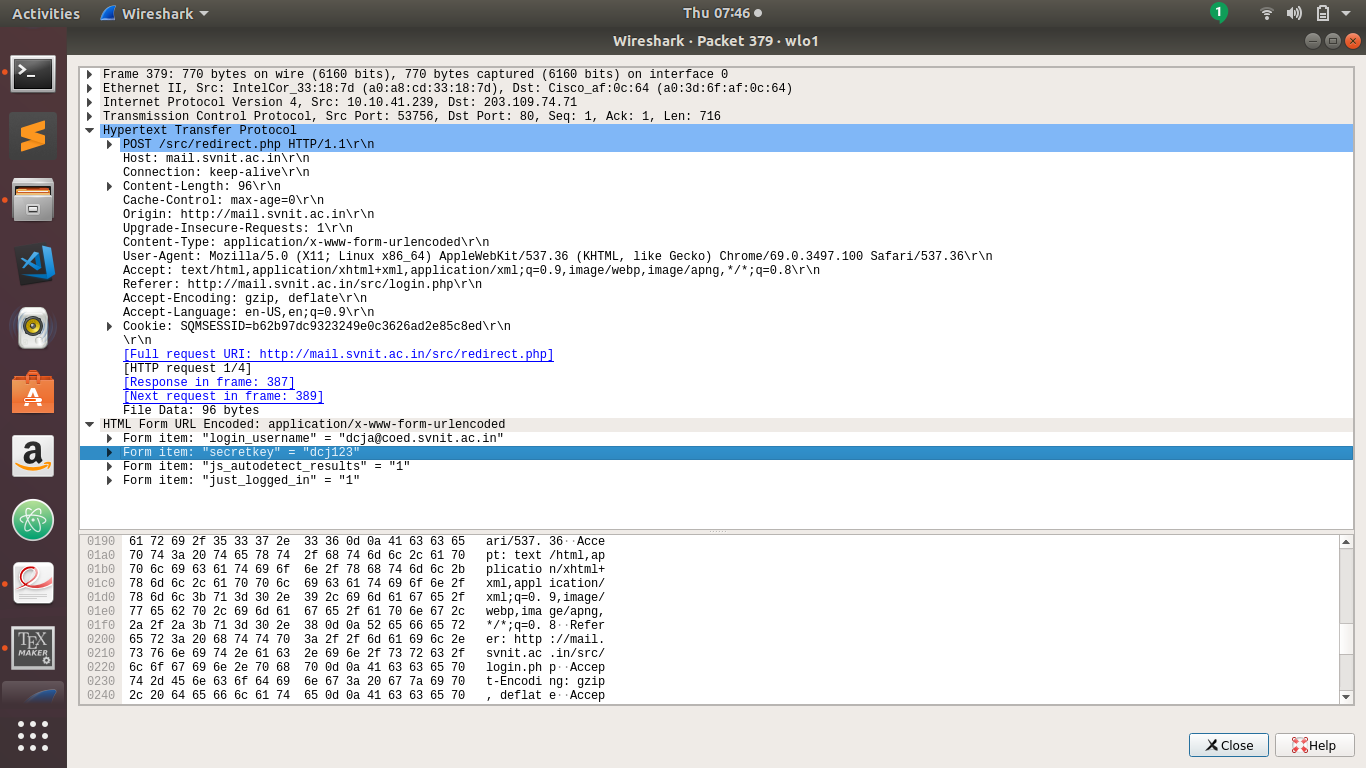
\includegraphics[width=0.8\textwidth]{../Set5/q3/a.png}
 \caption{\label{fig:PING}Screenshot of tcpdump file}
 \end{figure}

\end{document}